\documentclass[12pt]{article}
\usepackage{amsmath}
\usepackage{graphicx}
\usepackage{hyperref}
\usepackage{listings}
\usepackage{color}
\usepackage{pythonhighlight}

\title{Operating System Course Report - First Half of the Semester}
\author{A class}
\date{\today}

\begin{document}

\maketitle
\newpage

\tableofcontents
\newpage

\section{Introduction}
This report summarizes the topics covered during the first half of the Operating System course. It includes theoretical concepts, practical implementations, and assignments. The course focuses on the fundamentals of operating systems, including system architecture, process management, CPU scheduling, and deadlock handling.

\section{Course Overview}
\subsection{Objectives}
The main objectives of this course are:
\begin{itemize}
    \item To understand the basic components and architecture of a computer system.
    \item To learn process management, scheduling, and inter-process communication.
    \item To explore file systems, input/output management, and virtualization.
    \item To study the prevention and handling of deadlocks in operating systems.
\end{itemize}

\subsection{Course Structure}
The course is divided into two halves. This report focuses on the first half, which covers:
\begin{itemize}
    \item Basic Concepts and Components of Computer Systems
    \item System Performance and Metrics
    \item System Architecture of Computer Systems
    \item Process Description and Control
    \item Scheduling Algorithms
    \item Process Creation and Termination
    \item Introduction to Threads
    \item File Systems
    \item Input and Output Management
    \item Deadlock Introduction and Prevention
    \item User Interface Management
    \item Virtualization in Operating Systems
\end{itemize}

\section{Topics Covered}

\subsection{Basic Concepts and Components of Computer Systems}
This section explains the fundamental components that make up a computer system, including the CPU, memory, storage, and input/output devices.

\subsection{Performa Sistem dan Metrik Sistem Komputer}

\subsubsection{Performa Sistem}

\subsubsection{Metrik Sistem Utama}

\subsubsection{Metrik Sistem Spesifik}

\subsubsection{Pengukuran dan Optimasi Performa}

\par Performa sistem menjadi aspek penting yang mempengaruhi pengalaman pengguna serta efisiensi operasi. Untuk memastikan sistem berjalan optimal, perlu dilakukan pengukuran yang tepat terhadap berbagai komponen, serta optimasi yang berkelanjutan guna memperbaiki kinerja. Pengukuran performa membantu dalam memahami titik-titik lemah sistem, sementara optimasi bertujuan untuk meningkatkan efisiensi, mengurangi waktu respon, dan memaksimalkan penggunaan sumber daya.

\begin{enumerate}
    \item {Pengukuran performa}
        \par Pengukuran performa mengacu pada proses mengukur sejauh mana suatu sistem, aplikasi, atau proses memenuhi tujuan performa yang telah ditentukan. Hal ini sangat penting karena memberikan gambaran yang jelas mengenai efektivitas, efisiensi, dan kualitas suatu sistem atau aplikasi. Pengukuran ini melibatkan metrik seperti waktu respon, \textit{throughput}, dan penggunaan sumber daya (CPU, memori, jaringan). Hasil pengukuran dapat digunakan sebagai dasar untuk melakukan optimasi, identifikasi \textit{bottleneck}, serta perbaikan sistem yang lebih lanjut agar performa sistem dapat lebih stabil dan optimal dalam memenuhi kebutuhan pengguna.
        
        \begin{enumerate}
            \item \textit{Benchmarking}
            \par \textit{Benchmarking} adalah metode pengujian serangkaian program dengan cara membandingkan performa suatu sistem terhadap performa standar untuk mendapatkan performa relatif dari komponen PC atau sistem. Tujuan dari \textit{benchmarking} adalah untuk memberikan gambaran yang jelas tentang performa sistem komputer sehingga dapat dipastikan bahwa teknologi atau perangkat yang digunakan optimal dan memenuhi standar industri. Ada dua jenis dari \textit{benchmarking}:
            \begin{itemize}
                \item \textit{Synthetic benchmarking}: Simulasi skenario tertentu untuk mengukur potensi maksimum performa sistem, seperti menggunakan SPEC CPU untuk menguji kemampuan komputasi CPU.
                \item \textit{Real-world Benchmarking}: Pengukuran performa sistem menggunakan aplikasi nyata dalam kondisi operasional sehari-hari, seperti Adobe Premiere Pro untuk menguji kecepatan \textit{rendering} video.
            \end{itemize}
            
            \item \textit{Profiling}
            \par \textit{Profiling} adalah metode untuk menganalisis performa aplikasi atau sistem secara mendalam dengan fokus pada penggunaan sumber daya internal. \textit{Profiling} membantu mengidentifikasi bagian dari sistem atau program yang mengkonsumsi sumber daya paling banyak, seperti CPU, memori, I/O, dan waktu eksekusi. Dengan demikian, \textit{profiling} digunakan untuk menemukan dan memperbaiki "\textit{bottleneck}" dalam aplikasi atau sistem, memungkinkan pengembang untuk melakukan optimasi yang tepat. Berikut beberapa metode dalam \textit{profiling}:
            \begin{itemize}
                \item \textit{CPU profiling}: Mengukur penggunaan CPU untuk mengidentifikasi kode yang paling memakan waktu.
                \item \textit{Memory profiling}: Mengukur alokasi memori dan menemukan kebocoran memori. 
                \item \textit{I/O profiling}: Menganalisis performa operasi \textit{input}/\textit{output} seperti \textit{file} atau jaringan.
                \item \textit{Function-level profiling}: Menganalisis fungsi dalam aplikasi, melihat frekuensi pemanggilan dan durasi.
            \end{itemize}
            
            \item \textit{Monitoring}
            \par \textit{Monitoring} adalah proses pengamatan dan pengukuran performa sistem secara \textit{real-time} dan berkelanjutan untuk memastikan sistem berjalan optimal serta mendeteksi masalah atau potensi gangguan. \textit{Monitoring} sangat penting untuk menjaga stabilitas dan performa sistem komputer atau aplikasi, terutama dalam lingkungan produksi, di mana \textit{uptime} dan keandalan menjadi prioritas. Beberapa teknik yang sering digunakan dalam \textit{monitoring} antara lain:
            \begin{itemize}
                \item \textit{Real-time monitoring}:
                \par Memantau sistem secara langsung dan memberikan informasi performa atau kegagalan segera setelah terjadi. \textit{Real-time monitoring} sangat penting untuk aplikasi dengan kebutuhan \textit{uptime} tinggi, seperti layanan berbasis \textit{cloud}, sistem \textit{e-commerce}, atau \textit{server}.
                \item \textit{Historical monitoring}:
                \par Mengumpulkan data performa selama jangka waktu tertentu dan menyimpannya untuk dianalisis kemudian. Ini penting untuk analisis tren dan perencanaan kapasitas, karena memungkinkan tim IT untuk melihat bagaimana sistem telah beroperasi dalam jangka waktu tertentu.
                \item \textit{Threshold-based monitoring}:
                \par Sistem monitoring yang memberikan notifikasi ketika nilai performa melebihi atau di bawah batas tertentu. Misalnya, jika penggunaan CPU melebihi 90\% atau penggunaan memori terlalu rendah, sistem akan mengirimkan peringatan kepada administrator. Metode ini memungkinkan deteksi dini masalah performa dan membantu mencegah \textit{downtime} sistem. Selain CPU dan memori, \textit{threshold} juga dapat diterapkan pada metrik lain seperti penggunaan \textit{disk}, lalu lintas jaringan, atau waktu respons aplikasi. Administrator dapat menyesuaikan nilai ambang batas sesuai dengan kebutuhan spesifik sistem mereka.
            \end{itemize}
            
            \begin{table}[htbp]
            \centering
                \begin{tabular}{|p{2cm}|p{3cm}|p{3cm}|p{3cm}|}
                \hline
                Aspek & Benchmarking & Profiling & Monitoring \\
                \hline
                Fokus & Performa keseluruhan terhadap standar & Analisis mendalam per bagian sistem & Pemantauan performa \textit{real-time} \\
                \hline
                Tujuan & Perbandingan performa & Optimasi performa & Menjaga kestabilan sistem \\
                \hline
                Dilakukan saat & Di bawah kondisi spesifik (uji beban) & Saat pengembangan atau \textit{testing} & Selama sistem berjalan (operasional) \\
                \hline
                Hasil utama & Angka perbandingan & Identifikasi \textit{bottleneck} & Data penggunaan sumber daya \\
                \hline
                \end{tabular}
                \caption{Perbedaan dari \textit{Benchmarking}, \textit{Profiling}, dan \textit{Monitoring}}
                \label{table:ringkasan_perbedaan}
            \end{table}
        \end{enumerate}
            
    \item {Strategi Optimasi Performa}
        \begin{enumerate}
            \item Peningkatan \textit{hardware}
            \par Peningkatan \textit{hardware} mengacu pada peningkatan kapasitas fisik perangkat keras komputer untuk meningkatkan performa sistem. Beberapa cara peningkatan \textit{hardware} antara lain:
            \begin{itemize}
                \item Penambahan CPU/\textit{Core}: Meningkatkan eksekusi proses dan \textit{multitasking}.
                \item Penambahan RAM: Menjalankan lebih banyak aplikasi tanpa bergantung pada \textit{disk}.
                \item Penggunaan SSD: Mempercepat baca/tulis data dibanding HDD.
                \item Jaringan lebih Cepat: Mempercepat transfer data dengan \textit{bandwidth} tinggi.
            \end{itemize}
            
            \item Optimalisasi \textit{Software}
            \par Optimalisasi \textit{software} bertujuan untuk memaksimalkan efisiensi kode program dan cara perangkat lunak bekerja pada \textit{hardware} yang tersedia. Berikut adalah beberapa langkah untuk mengoptimalkan \textit{software}:
            \begin{itemize}
                \item Optimalisasi algoritma: Mengurangi kompleksitas untuk mempercepat proses.
                \item \textit{Caching}: Menyimpan data sering diakses untuk mempercepat.
                \item \textit{Database tuning}: Indeksasi dan optimasi \textit{query} untuk eksekusi lebih cepat.
                \item Kompresi data: Mengurangi ukuran data untuk transfer lebih cepat.
                \item Pengurangan \textit{latency}: Menggunakan CDN untuk akses lebih cepat.
            \end{itemize}
            
            \item \textit{Load balancing}
            \par \textit{Load balancing} adalah teknik distribusi beban kerja di beberapa \textit{server} atau sumber daya untuk memastikan bahwa tidak ada satu \textit{server} yang kelebihan beban, sementara \textit{server} lainnya tidak terpakai secara maksimal. \textit{Load balancing} dapat diterapkan pada sistem yang berbasis \textit{server} untuk aplikasi \textit{web}, basis data, atau layanan \textit{cloud}.
            \begin{figure}[h]
                \centering
                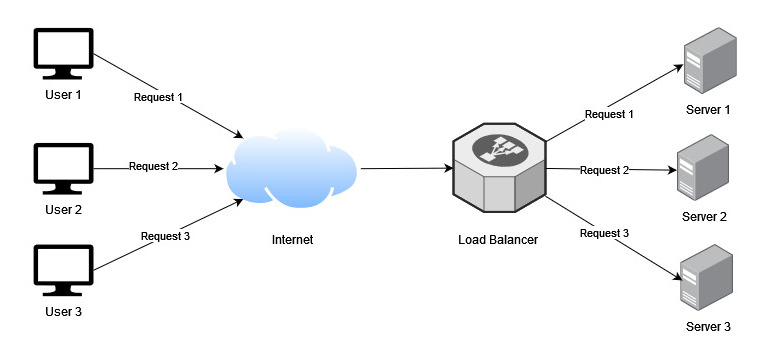
\includegraphics[width=0.7\textwidth] {asset/proses_load_balancing.jpg} 
                \caption{Ilustrasi proses \textit{load balancing}}
                \label{fig:proses_load_balancing}
            \end{figure}
            \par Pada gambar \ref{fig:proses_load_balancing}, tiga pengguna (\textit{User} 1, \textit{User} 2, \textit{User} 3) mengirimkan permintaan melalui \textit{internet}. Permintaan tersebut didistribusikan oleh \textit{load balancer} ke beberapa \textit{server} (\textit{Server} 1, \textit{Server} 2, \textit{Server} 3), memastikan beban kerja tersebar merata dan tidak ada \textit{server} yang kelebihan beban.
        \end{enumerate}
\end{enumerate}

\subsection{System Architecture of Computer Systems}
Describes the architecture of modern computer systems, focusing on the interaction between hardware and the operating system.

\subsection{Process Description and Control}
Processes are a central concept in operating systems. This section covers:
\begin{itemize}
    \item Process states and state transitions
    \item Process control block (PCB)
    \item Context switching
\end{itemize}

\subsection{Scheduling Algorithms}
This section covers:
\begin{itemize}
    \item First-Come, First-Served (FCFS)
    \item Shortest Job Next (SJN)
    \item Round Robin (RR)
\end{itemize}
It explains how these algorithms are used to allocate CPU time to processes.

\subsection{Process Creation and Termination}
Details how processes are created and terminated by the operating system, including:
\begin{itemize}
    \item Process spawning
    \item Process termination conditions
\end{itemize}

\subsection{Introduction to Threads}
This section introduces the concept of threads and their relation to processes, covering:
\begin{itemize}
    \item Single-threaded vs. multi-threaded processes
    \item Benefits of multithreading
\end{itemize}

\begin{figure}[h]
    \centering
    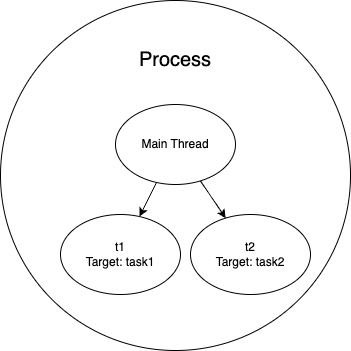
\includegraphics[width=0.5\textwidth]{/Users/khawaritzmi/Unhas/os_report_mid2024/a_class/asset/example.png}  % Sesuaikan nama file dan ukurannya
    \caption{Ini adalah gambar contoh dari multithreading.}
    \label{fig:contoh_gambar}
\end{figure}

Seperti yang terlihat pada Gambar \ref{fig:contoh_gambar}, inilah cara menambahkan gambar dengan keterangan.

\subsection{File Systems}
File systems provide a way for the operating system to store, retrieve, and manage data. This section explains:
\begin{itemize}
    \item File system structure
    \item File access methods
    \item Directory management
\end{itemize}

\subsection{Input and Output Management}
Input and output management is key for handling the interaction between the system and external devices. This section includes:
\begin{itemize}
    \item Device drivers
    \item I/O scheduling
\end{itemize}

\subsection{Deadlock Introduction and Prevention}
Explores the concept of deadlocks and methods for preventing them:
\begin{itemize}
    \item Deadlock conditions
    \item Deadlock prevention techniques
\end{itemize}

\subsection{User Interface Management}
This section discusses the role of the operating system in managing the user interface. Topics covered include:
\begin{itemize}
    \item Graphical User Interface (GUI)
    \item Command-Line Interface (CLI)
    \item Interaction between the user and the operating system
\end{itemize}

\subsection{Virtualization in Operating Systems}
Virtualization allows multiple operating systems to run concurrently on a single physical machine. This section explores:
\begin{itemize}
    \item Concept of virtualization
    \item Hypervisors and their types
    \item Benefits of virtualization in modern computing
\end{itemize}

\section{Assignments and Practical Work}
\subsection{Assignment 1: Process Scheduling}
Students were tasked with implementing various process scheduling algorithms (e.g., FCFS, SJN, and RR) and comparing their performance under different conditions.
\subsubsection{Group 1}
\begin{python}
    class Process:
    def __init__(self, pid, arrival_time, burst_time):
        self.pid = pid
        self.arrival_time = arrival_time
        self.burst_time = burst_time
        self.completion_time = 0
        self.turnaround_time = 0
        self.waiting_time = 0
\end{python}

\begin{table}[htbp] % Optional: For floating position
    \centering
    \begin{tabular}{|c|c|c|} % Defines number of columns and alignment (c = center, l = left, r = right). '|' creates vertical lines.
    \hline
    Header 1 & Header 2 & Header 3 \\ % Column headers
    \hline
    Row 1, Column 1 & Row 1, Column 2 & Row 1, Column 3 \\ % First row of data
    \hline
    Row 2, Column 1 & Row 2, Column 2 & Row 2, Column 3 \\ % Second row of data
    \hline
    \end{tabular}
    \caption{Your table caption} % Optional: For adding a caption
    \label{tab:your_label} % Optional: For cross-referencing the table
\end{table}
\subsection{Assignment 2: Deadlock Handling}
In this assignment, students were asked to simulate different deadlock scenarios and explore various prevention methods.

\subsection{Assignment 3: Multithreading and Amdahl's Law}
This assignment involved designing a multithreading scenario to solve a computationally intensive problem. Students then applied **Amdahl's Law** to calculate the theoretical speedup of the program as the number of threads increased.

\subsection{Assignment 4: Simple Command-Line Interface
(CLI) for User Interface Management}
\subsubsection{Group 2}
\textbf{Soal:}
\par Buatlah sebuah program Python sederhana yang berfungsi sebagai \textit{Command-Line Interface} (CLI) untuk manajemen antarmuka pengguna. Program ini harus mendukung beberapa perintah dasar, seperti manipulasi \textit{file} (membuat, menampilkan daftar, dan menghapus \textit{file}), manajemen proses, dan pelaporan status sistem. Berikut adalah ketentuan-ketentuan dari program yang harus dibuat:
\begin{itemize}
    \item Buat \textit{file} dengan nama tertentu.
    \item Tampilkan daftar \textit{file} dalam direktori saat ini.
    \item Hapus \textit{file} berdasarkan nama \textit{file}.
    \item Tampilkan daftar proses yang sedang berjalan.
    \item Tampilkan status penggunaan CPU dan memori saat ini.
\end{itemize}
\textbf{Jawaban:}
\par Untuk menjawab soal ini, kita akan membuat program Python sederhana yang berfungsi sebagai \textit{Command-Line Interface} (CLI) untuk manajemen \textit{interface} pengguna. Program ini akan mendukung beberapa fitur utama seperti manipulasi \textit{file}, manajemen proses, dan pelaporan status sistem. Berikut adalah implementasi program tersebut:
\begin{python}
    import os
    import psutil
    
    def tampilkan_welcome_screen():
        print(
            """
        \033[32m ___  ___      _____ _     _____\033[0m
        \033[32m|  \/  |     /  __ \ |   |_   _|\033[0m
        \033[32m| .  . |_   _| /  \/ |     | |  \033[0m
        \033[32m| |\/| | | | | |   | |     | |  \033[0m
        \033[32m| |  | | |_| | \__/\ |_____| |_ \033[0m
        \033[32m\_|  |_/\__, |\____/\_____/\___/\033[0m
        \033[32m         __/ |                  \033[0m
        \033[32m        |___/                   \033[0m
    
        \033[35mPenggunaan: python mycli.py\033[0m
    
        \033[36mMengelola file dan menampilkan informasi sistem\033[0m
        """)
    
    def tampilkan_daftar_file():
        try:
            files = os.listdir('.')
            print("Daftar file:", ", ".join(files) if files else "Tidak ada file")
        except Exception as e:
            print(f"Gagal menampilkan daftar file: {e}")
    
    def tampilkan_daftar_proses():
        try:
            for proc in psutil.process_iter(['pid', 'name']):
                print(f"PID: {proc.info['pid']}, Nama: {proc.info['name']}")
        except Exception as e:
            print(f"Gagal menampilkan daftar proses: {e}")
    
    def tampilkan_status_sistem():
        try:
            cpu = psutil.cpu_percent()
            mem = psutil.virtual_memory()
            print(f"CPU: {cpu}%, RAM: {mem.percent}% ({mem.used/1e9:.1f}/{mem.total/1e9:.1f} GB)")
        except Exception as e:
            print(f"Gagal menampilkan status sistem: {e}")
    
    def main():
        tampilkan_welcome_screen()
        
        perintah = {
            '1': ('Buat file', 
                    lambda: open(input("Nama file: "), 'w').close()),
            '2': ('Tampilkan daftar file', 
                    tampilkan_daftar_file),
            '3': ('Hapus file', 
                    lambda: os.remove(input("Nama file: "))),
            '4': ('Tampilkan daftar proses', 
                    tampilkan_daftar_proses),
            '5': ('Tampilkan status sistem', 
                    tampilkan_status_sistem),
            '6': ('Keluar', 
                    exit)
        }
        
        while True:
            print("\n" + "\n".join(f"{k}. {v[0]}" for k, v in perintah.items()))
            try:
                perintah[input("Pilih perintah: ")][1]()
            except Exception as e:
                print(f"Error: {e}")
    
    if __name__ == "__main__":
        main()
\end{python}
\par Hasil \textit{output}:
\begin{figure}[h]
    \centering
    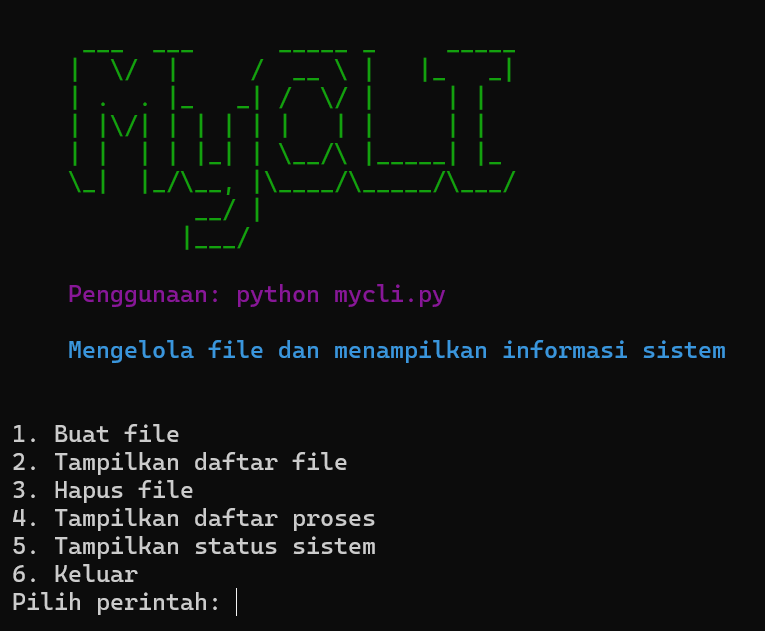
\includegraphics[width=0.5\textwidth] {asset/output_assignment4_group2.png} 
    \caption{\textit{output assignment} 4}
    \label{fig:output_assignment_4}
\end{figure}

\subsection{Assignment 5: File System Access}
In this assignment, students implemented file system access routines, including:
\begin{itemize}
    \item File creation and deletion
    \item Reading from and writing to files
    \item Navigating directories and managing file permissions
\end{itemize}

\section{Conclusion}
The first half of the course introduced core operating system concepts, including process management, scheduling, multithreading, and file system access. These topics provided a foundation for more advanced topics to be covered in the second half of the course.

\begin{thebibliography}{3}
    \bibitem{3.2.4Altvater2023}
    Altvater, A. (2023). \textit{What is code profiling? learn the 3 types of code profilers.} Stackify. Diakses pada 1 oktober 2024, dari https://stackify.com/what-is-code-profiling/ 
    
    \bibitem{3.2.4Bhat2021}
    Bhat, A. (2021). \textit{Benchmarking in computer.}Benchmarking in computer. Medium. Diakses pada 1 oktober 2024, dari https://bhatabhishek-ylp.medium.com/benchmarking-in-computer-c6d364681512 

    \bibitem{3.2.4GeeksforGeeks2024}
    GeeksforGeeks. (2024). \textit{Performance of computer in Computer Organization.} Diakses pada 1 oktober 2024, dari https://www.geeksforgeeks.org/computer-organization-performance-of-computer/ 
\end{thebibliography}
\end{document}